\chapter{\texttt{NP} completezza e \texttt{co-NP}}
\section{Classi di complessità}
L'idea fondamentale per dimostrare che determinati problemi sono più difficili dei problemi 
risolvibili in tempo polinomiale è quella di ``ritagliare'' una classe di problemi
che abbiano una determinata caratteristica, e dimostrare che un problema specifico
è almeno tanto difficile quanto i problemi di quella classe, \textbf{riducendo} il problema
specifico ad un problema della classe.
\subsection{Tipologie di problemi}
\begin{itemize}
    \item \textbf{Problemi decisionali}: problemi che ammettono risposta
    sì/no. Un problema di decisione è quindi un insieme di istanze, e la risposta
    è sì se l'istanza appartiene all'insieme, no altrimenti.

    \textit{Un problema di decisione è il seguente: dato un grafo $\mathcal{G}$ dire se 
    esiste un cammino euleriano in $\mathcal{G}$.}

    \item \textbf{Problemi di ricerca}: problemi di ricerca ammettono una soluzione
    che può essere trovata in tempo polinomiale.

    \textit{Un problema di ricerca è il seguente: dato un grafo $\mathcal{G}$
    trovare un cammino euleriano in $\mathcal{G}$.}
            
    \item \textbf{Problemi di ottimizzazione}: problemi di ottimizzazione
    ammettono una soluzione che può essere trovata in tempo polinomiale.

    \textit{Un problema di ottimizzazione è il seguente: dato un grafo $\mathcal{G}$
    trovare il cammino euleriano più lungo in $\mathcal{G}$.}
\end{itemize}
Nello studio della complessità considereremo solo problemi decisionali, in quanto
tutti i problemi di ricerca e di ottimizzazione possono essere ricondotti a problemi
di decisione. Ciò significa che se siamo in grado di dire che un determinato problema
di decisione è difficile, allora possiamo dire che anche il problema di ricerca e
quello di ottimizzazione sono difficili, perché se fossimo in grado di risolvere un 
problema di ricerca o di ottimizzazione, potremmo risolvere anche il problema di decisione
in tempo polinomiale.
\subsection{Formalizzazione di un problema computazionale}
In relazione a ciò che è stato detto nella sezione \ref{sec:problema_computazionale}, 
un problema computazionale è un insieme infinito di istanze e la loro relazione con
la soluzione associata. Matematicamente, possiamo definire un problema computazionale
attraverso:
\begin{itemize}
    \item $\mathbb{A}$ denota il problema computazionale sotto esame.
    \item $\mathscr{I}(\mathbb{A})$ rappresenta lo spazio delle istanze,
    ovvero il dominio dei possibili quesiti.
    \item $\texttt{sol}(\mathbb{A})$ esprime la relazione che associa a
    ciascuna istanza la sua soluzione o insieme di soluzioni.
\end{itemize}

\begin{exmp}
Consideriamo, ad esempio, il problema del ciclo hamiltoniano. In questo contesto:
    \begin{itemize}
        \item $\mathbb{A}$ corrisponde alla questione di determinare l'esistenza
        di un ciclo hamiltoniano.
        \item $\mathscr{I}(\mathbb{A})$ comprende tutti i possibili grafi $\mathcal{G}$
        sui quali indaghiamo.
        \item $\texttt{sol}(\mathbb{A})$ identifica i percorsi che visitano ogni nodo del
        grafo esattamente una volta, se esistenti.
    \end{itemize}
\end{exmp}

Pertanto, la relazione $\mathbb{A}$ si configura come una \textbf{connessione} fra lo
spazio delle istanze e le corrispondenti soluzioni. Matematicamente, ciò si traduce
nella seguente inclusione:
\[ \mathbb{A} \subseteq \mathscr{I}(\mathbb{A}) \times \texttt{sol}(\mathbb{A}) \]
indicando con $(\mathcal{G}, \mathcal{P})$ l'insieme delle coppie dove $\mathcal{P}$
rappresenta un valido ciclo hamiltoniano nel grafo $\mathcal{G}$.

Per ciascuna istanza $x$ appartenente allo spazio dei problemi computazionali,
$\texttt{sol}(x)$ denota l'insieme delle soluzioni $y$ tali che $(x, y) \in \mathbb{A}$,
ovvero:
\[
    \texttt{sol}(x) = \{ y \mid (x, y) \in \mathbb{A} \}
\]

\subsubsection{Problemi di Decisione}
Nei problemi di decisione, lo spazio delle soluzioni è binario, $\texttt{sol}(\mathbb{A})
= \{ \texttt{yes}, \texttt{no} \}$. Pertanto, $A$ associa a ciascuna istanza $x$ una delle
due possibili risposte, determinando se l'istanza soddisfa la proprietà esaminata:
\[
    A : \mathscr{I}(\mathbb{A}) \rightarrow \{ \texttt{yes}, \texttt{no} \}
\]

\subsubsection{Problemi di Ricerca}
Per i problemi di ricerca $\mathbb{A}^S$, il problema di decisione associato $\mathbb{A}^D$
verifica l'esistenza di almeno una soluzione per l'istanza $x$:
\[
    \mathbb{A}^D(x) = 
    \begin{cases}
        \texttt{yes} & \text{se esiste almeno una soluzione}, \\
        \texttt{no} & \text{altrimenti}
    \end{cases}
\]

\subsection{La Classe \texttt{P}}

Nella teoria della complessità computazionale, la capacità di risolvere un problema
computazionale va oltre la semplice identificazione di una soluzione per un'istanza
specifica. Ciò richiede l'impiego di un algoritmo deterministico $A$ che, per ogni istanza
$x$ nell'insieme $\mathscr{I}(\mathbb{A})$, produce una soluzione $y$ valida, ovvero $y
\in \texttt{sol}(x)$:
\[
  A(x) = y \quad \text{con} \quad y \in \texttt{sol}(x)
\]

Il \textit{tempo di esecuzione} $T_A(x)$ dell'algoritmo $A$ su un'istanza $x$ è fondamentale,
poiché riflette l'efficienza con cui l'algoritmo raggiunge la soluzione.

\begin{tcolorbox}[title={Classe \texttt{P}}]
Un algoritmo $A$ è definito \textit{polinomiale} (\texttt{poly-time}) quando il suo tempo di
esecuzione, per ogni istanza $x \in \mathscr{I}(\mathbb{A})$, è limitato superiormente da
un polinomio nella dimensione di $x$:
\[
    T_A(x) = O(|x|^c) \quad \text{per una certa costante } c \in \mathbb{N}.
\]
\end{tcolorbox}

Un problema computazionale viene considerato \textit{fuori dalla classe \texttt{P}} qualora
non esista, per nessuna costante $c$, un algoritmo capace di risolvere tutte le sue istanze
in tempo polinomiale $O(n^c)$.

\subsection{La Classe \texttt{EXP}}
\begin{tcolorbox}[title={Classe \texttt{EXP}}]
    La classe \texttt{EXP} raggruppa i problemi di decisione risolvibili da un algoritmo
    deterministico in tempo esponenziale rispetto
    alla dimensione dell'input. Un problema $\mathbb{A}$ appartiene a \texttt{EXP} se
    esiste un algoritmo $A$ per cui, data una costante $c_A$, per ogni istanza $x \in
    \mathscr{I}(\mathbb{A})$ si ha che:
    \[
        T_A(x) = O(2^{|x|^{c_A}})
    \]
    In altre parole, il tempo di esecuzione di $A$ è limitato superiormente da una
    funzione esponenziale della dimensione dell'input elevata a una costante. Questa
    classe include quindi problemi per i quali la risoluzione richiede una quantità di
    tempo che cresce esponenzialmente con l'aumentare della dimensione dell'input.
\end{tcolorbox}
Da qui segue che la classe \texttt{EXP} è una generalizzazione della classe \texttt{P},
poiché ogni problema risolvibile in tempo polinomiale è anche risolvibile in tempo
esponenziale. In altre parole, \texttt{P} è un sottoinsieme di \texttt{EXP}.
\[ \texttt{P} \subseteq \texttt{EXP} \]
Perché se un problema $\mathcal{A} \in \texttt{P}$, allora esiste un algoritmo $A$, 
per cui, data una costante $c_A$, per ogni istanza $x \in \mathscr{I}(\mathbb{A})$ si ha che:
\[ T_A(x) = O(|x|^{c_A}) \]
Poiché, ogni polinomio è anche una funzione esponenziale, si ha che:
\[ T_A(x) = O(2^{|x|^{c_A}}) \]
Quindi $\mathbb{A} \in \texttt{EXP}$.

È importante notare che un problema è nella classe \texttt{EXP}, non se gli unici 
algoritmi conosciuti per risolverlo sono esponenziali, ma se esiste almeno un algoritmo
deterministico che lo risolve in tempo esponenziale.
\begin{exmp}
    Consideriamo il problema del cammino euleriano. Un cammino euleriano è un cammino che
    attraversa ogni arco del grafo esattamente una volta. 
    In input si ha un grafo $\mathcal{G}$ e si vuole sapere se esiste un cammino euleriano
    in $\mathcal{G}$, quindi l'output è \texttt{yes} se esiste un cammino euleriano e
    \texttt{no} altrimenti. 
    Questo problema è nella classe \texttt{P}, infatti esiste un algoritmo polinomiale
    per risolverlo, controllando se il grafo è connesso e se ogni nodo ha grado pari.
\end{exmp}
\begin{exmp}
    Consideriamo il problema del commesso viaggiatore. In input si ha un grafo completo
    pesato $\mathcal{G}$ e si vuole sapere se esiste un ciclo hamiltoniano di peso minimo
    in $\mathcal{G}$, quindi l'output è \texttt{yes} se esiste un ciclo hamiltoniano e
    \texttt{no} altrimenti. 
    Non sappiamo se esiste un algoritmo polinomiale per risolvere questo problema, quindi
    non sappiamo se è nella classe \texttt{P}. Sappiamo che per ogni istanza, se la soluzione 
    è \texttt{yes} possiamo certificarla in tempo polinomiale. 
\end{exmp}

\begin{tcolorbox}[title={Prova Semplice}]
    Una \textbf{prova semplice} è un certificato di lunghezza polinomiale che può essere
    verificato in tempo polinomiale. 
\end{tcolorbox}
Cerchiamo di caratterizzare i problemi che hanno una prova semplice.
\subsection{La Classe \texttt{NP}}

\begin{tcolorbox}[title = {Classe \texttt{NP}}]
    Un problema $\mathbb{A}$ appartiene alla classe \texttt{NP} se esiste un algoritmo
    deterministico $A$ (\textit{verificatore}) e una funzione polinomiale $p$ tale che, per ogni istanza $x \in
    \mathscr{I}(\mathbb{A})$, esiste un certificato $y$ di lunghezza polinomiale rispetto
    alla dimensione di $x$ tale che:
    \[
        B(x, y) = \begin{cases}
            \texttt{yes} & \text{se } x \in \texttt{sol}(\mathbb{A}), \\
            \texttt{no} & \text{altrimenti}
        \end{cases}
    \]

    Inoltre, esiste una costante $c_A$ tale che il tempo di esecuzione di $A$ è limitato
    superiormente da una funzione polinomiale della dimensione di $x$:
    \[
        T_A(x, y) = O(p(|x|^{c_A}))
    \]

    In notazione formale, si ha che:
    \begin{align*}
        \texttt{NP} = \{ &\mathbb{A} \mid \exists A, c_A,
        \forall x \in \mathscr{I}(\mathbb{A}): \mathbb{A}(x) = \texttt{yes} \Rightarrow \\
        &\exists y, |y| = O((|x|^{c_A})), \text{ t.c. } A(x, y) = \texttt{yes} \land T_A(x, y) 
        = O((|x|^{c_A})) \}
    \end{align*}
\end{tcolorbox}
È importante notare che il tempo di esecuzione del verificatore $A$ è polinomiale rispetto 
alla dimensione dell'input $x$ e del certificato $y$. Ciò significa che, se esiste un
certificato $y$ tale che $A(x, y) = \texttt{yes}$, allora esiste un algoritmo che può
verificare la soluzione in tempo polinomiale. Da questo segue che il certificato deve 
essere di lunghezza polinomiale rispetto alla dimensione dell'input $x$.
\[
    |y| = O((|x|^{c_A}))  
\]

\begin{theorem}
    La classe \texttt{P} è un sottoinsieme della classe \texttt{NP}.
    \[
        \texttt{P} \subseteq \texttt{NP}.
    \]
\end{theorem}
\begin{proof}
    Consideriamo il problema $\mathbb{A} \in \texttt{P}$. Allora esiste un algoritmo 
    deterministico $A$ che risolve per ogni istanza $x \in \mathscr{I}(\mathbb{A})$ in
    tempo polinomiale:
    \[
        T_A(x) = O(|x|^{c_A}).
    \]
    Definiamo un verificatore $B$ per $\mathbb{A}$. Per ogni istanza
    $x \in \mathscr{I}(\mathbb{A})$ e $y$, $B(x, y) = A(x)$. 
    Quindi se $\mathbb{A}(x) = \texttt{yes}$, allora per ogni $y \in \{0,1\}^*$,
    $B(x, y) = \texttt{yes}$ e se $\mathbb{A}(x) = \texttt{no}$, allora per ogni
    $y \in \{0,1\}^*$, $B(x, y) = \texttt{no}$.
\end{proof}

\begin{theorem}
    La classe \texttt{NP} è sottoinsieme della classe \texttt{EXP}.
    \[
        \texttt{NP} \subseteq \texttt{EXP}.
    \]
\end{theorem}
\begin{proof}
    Consideriamo un problema $\mathbb{A} \in \texttt{NP}$. Allora esiste un algoritmo
    deterministico $B$ e una costante $c_B$ tale che per ogni istanza $x \in
    \mathscr{I}(\mathbb{A})$, esiste un certificato $y$ di lunghezza polinomiale rispetto
    alla dimensione di $x$ tale che:
    \[
        B(x, y) = \begin{cases}
            \texttt{yes} & \text{se } x \in \texttt{sol}(\mathbb{A}), \\
            \texttt{no} & \text{altrimenti}.
        \end{cases}
    \]
    Quindi il tempo di esecuzione di $B$ è limitato superiormente da una funzione polinomiale
    della dimensione di $x$:
    \[
        T_B(x, y) = O((|x|^{c_B}))
    \]
    Definiamo un algoritmo deterministico $A^{\texttt{EXP}}$ che per ogni 
    $x \in \mathscr{I}(\mathbb{A})$ cicla su tutti i possibili certificati $y$ della 
    taglia ammissibile per i certificati e usa $B(x, y)$ per verificare se $x$ è 
    una soluzione di $\mathbb{A}$:

    \begin{algorithm}[H]
        \DontPrintSemicolon
        \caption{Algoritmo $A^{\texttt{EXP}}$}
        \KwIn{Un'istanza $x \in \mathscr{I}(\mathbb{A})$}
        \KwOut{\texttt{yes} se $x \in \texttt{sol}(\mathbb{A})$, \texttt{no} altrimenti}
        \ForEach{$y \in \{0,1\}^{|x|^{c_B}}$}{
            \If{$B(x, y) = \texttt{yes}$}{
                \Return{\texttt{yes}}
            }
            \Return{\texttt{no}}
        }
    \end{algorithm}
    Sappiamo che $A^{\texttt{EXP}}(x) = \texttt{yes}$ se e solo se esiste un certificato
    $y \in \{0,1\}^{|x|^{c_B}}$ tale che $B(x, y) = \texttt{yes}$, ovvero se 
    $\mathbb{A} = \texttt{yes}$. Il tempo di esecuzione di $A^{\texttt{EXP}}$ è limitato
    superiormente da una funzione esponenziale della dimensione di $x$:
    \[
        T_{A^{\texttt{EXP}}}(x) = O(2^{|x|^{c_B}})
    \]
    Quindi $\mathbb{A} \in \texttt{EXP}$, ovvero $\texttt{NP} \subseteq \texttt{EXP}$.
\end{proof}

\begin{figure}[H]
    \centering
    \cclasses{\texttt{EXP}, \texttt{NP}, \texttt{P}}
\end{figure}
Non sappiamo se le inclusioni sono strette, ma sappiamo che \texttt{P} è incluso
strettamente in \texttt{EXP}.

\begin{tcolorbox}[title = {Congettura $\texttt{P} \neq \texttt{NP}$}]
    Se $\texttt{P} \neq \texttt{NP}$, quindi $\texttt{P} \subset \texttt{NP}$, allora
    esistono problemi che possono essere verificati in tempo polinomiale, ma non possono
    essere risolti in tempo polinomiale.
    \begin{align*}
        \texttt{P} &\subset \texttt{NP} \\
        \texttt{P} &\neq \texttt{NP}
    \end{align*}
    Il problema è che non esiste una dimostrazione formale che 
    $\texttt{P} \neq \texttt{NP}$. Siamo convinti di ciò perché crediamo che alcuni
    problemi \texttt{NP} siano
    più difficili di altri e se siamo in grado di risolvere tali problemi allora 
    siamo in grado di risolvere tutti i problemi \texttt{NP}. Questa situazione
    porta alla distinzione tra i problemi \texttt{NP} cosiddetti ``difficili" o
    \texttt{NP-hard} e i problemi \texttt{NP-completi}, per i quali una soluzione
    efficiente implicherebbe la possibilità di risolvere efficientemente ogni problema
    nell'insieme \texttt{NP}.

\end{tcolorbox}
\begin{figure}[H]
    \centering
    \begin{tikzpicture}[set/.style={draw, circle, inner sep=0pt, align=center}]
        \node[set, fill=gray!40, text width=2.5cm] (P) at (0,0) {Problemi \texttt{P}};
        \node[set, fill=gray!40, text width=2.5cm] (NP) at (3,0) {\texttt{NP}-Completi};
        \begin{pgfonlayer}{background}
            \node[fill=gray!20, fit=(P) (NP), draw, rounded corners=0.5cm, inner
            sep=0.5cm, label={above: Problemi \texttt{NP}}] {};
        \end{pgfonlayer}
    \end{tikzpicture}
\end{figure}
\section{Riduzione polinomiale tra problemi}
La riduzione polinomiale ci permette di mettere in relazione i problemi tra loro, 
permettendoci di dimostrare che un problema è almeno tanto difficile quanto un altro
problema.
\begin{tcolorbox}[title = {Riduzione polinomiale (Karp)}]
    Siano $\mathbb{A}$ e $\mathbb{B}$ due problemi decisionali. Diciamo che $\mathbb{A}$
    si riduce polinomialmente a $\mathbb{B}$, e scriviamo $\mathbb{A} \leq_p \mathbb{B}$,
    se esiste una funzione calcolabile in tempo polinomiale $f: \{0,1\}^* \rightarrow
    \{0,1\}^*$ tale che per ogni $x \in \{0,1\}^*$:
    \[
        \forall x \in \mathbb{A} \qquad \mathbb{A}(x) = \texttt{yes} \iff \mathbb{B}(f(x)) = \texttt{yes}
    \]
\end{tcolorbox}
\subsection{Colorazione di un grafo}
Consideriamo il problema della colorazione di un grafo. Dato un grafo $\mathcal{G} = (V, E)$,
dove $V$ è l'insieme dei vertici e $E$ è l'insieme degli archi, il problema consiste
nel determinare se è possibile colorare i vertici di $\mathcal{G}$ con $k$ colori in modo che
due vertici adiacenti non abbiano lo stesso colore. Solitamente tale problema si associa 
al problema di allocazione di risorse, dove i vertici rappresentano le risorse e gli archi
rappresentano le relazioni di dipendenza tra le risorse.

\begin{tcolorbox}
    La coloriazione è \textbf{propria} se per ogni arco $(u, v) \in E$ si ha che
    $c(u) \neq c(v)$, ovvero due vertici adiacenti non possono avere lo stesso colore.
\end{tcolorbox}
Il problema della \texttt{k-colorazione} è un problema \texttt{NP} perché possiamo
verificare in tempo polinomiale se una colorazione è propria. Quindi una \textbf{prova semplice} 
che dimostra che il problema della \texttt{k-colorazione} è \texttt{NP} è la seguente:
\begin{itemize}
    \item Dato un grafo $\mathcal{G}$ e una colorazione $c: V \rightarrow \{1, \ldots, k\}$,
    possiamo verificare in tempo polinomiale se $c$ è una colorazione propria, e tale 
    colorazione si verifica in tempo polinomiale $O(|V| + |E|)$.
    Immaginiamo che la colorazione sia una funzione che associa ad ogni vertice un numero 
    intero che rappresenta il colore del vertice. Se $c$ è una colorazione propria, allora
    per ogni arco $(u, v) \in E$ si ha che $c(u) \neq c(v)$.
\end{itemize}

Ci chiediamo ora se esiste un algoritmo polinomiale per la colorazione di un grafo.
La risposta è legata al parametro $k$ che rappresenta la diversa tipologia di 
problemi che possiamo avere. Proviamo a vedere per i diversi valori di $k$ se esiste
un algoritmo polinomiale per la colorazione di un grafo:
\begin{itemize}
    \item \textbf{k = 1}: se $k = 1$ allora il problema è banale, perché tutti i vertici
    devono avere lo stesso colore, per farlo basta che il grafo sia massimamente disconnesso,
    ovvero non ci siano archi tra i vertici. Questo problema è risolvibile in tempo polinomiale.
    \item \textbf{k = 2}: se $k = 2$ allora il problema è equivalente al problema della
    \texttt{bipartizione} di un grafo, ovvero se è possibile dividere i vertici di un grafo
    in due insiemi $V_1$ e $V_2$ tali che non esistano archi tra vertici dello stesso insieme.
    Per verificare che un grafo è bipartito possiamo verificare che non esistano cicli dispari
    nel grafo. Questo problema è risolvibile in tempo polinomiale, infatti possiamo utilizzare
    l'algoritmo di \texttt{BFS}, che ha complessità $O(|V| + |E|)$.
\end{itemize}
Per $k \geq 3$ non sappiamo se esiste un algoritmo polinomiale per la colorazione di un grafo.

\begin{tcolorbox}[title = {$\texttt{k-colorazione} \leq_p \texttt{(k + 1)-colorazione}$}]
    Se \texttt{(k+1)-colorazione} è \texttt{P}, allora \texttt{k-colorazione} è \texttt{P},
    ovvero \texttt{(k+1)-colorazione} non è più facile di \texttt{k-colorazione}.
    \[
      \texttt{(k+1)-col} \in \texttt{P} \implies \texttt{k-col} \in \texttt{P} 
      \equiv \texttt{k-col} \not \in \texttt{P} \implies \texttt{(k+1)-col} \not \in \texttt{P}
    \]
\end{tcolorbox}
\begin{proof}
    Forniamo la funzione calcolabile in tempo polinomiale $f$, 
    tale che per ogni grafo $\mathcal{G}$, se $\mathcal{G}$ è un grafo \texttt{k-colorabile},
    se e solo se $f(\mathcal{G})$ è un grafo
    \texttt{(k+1)-colorabile}. 

    \begin{figure}[H]
        \centering 
        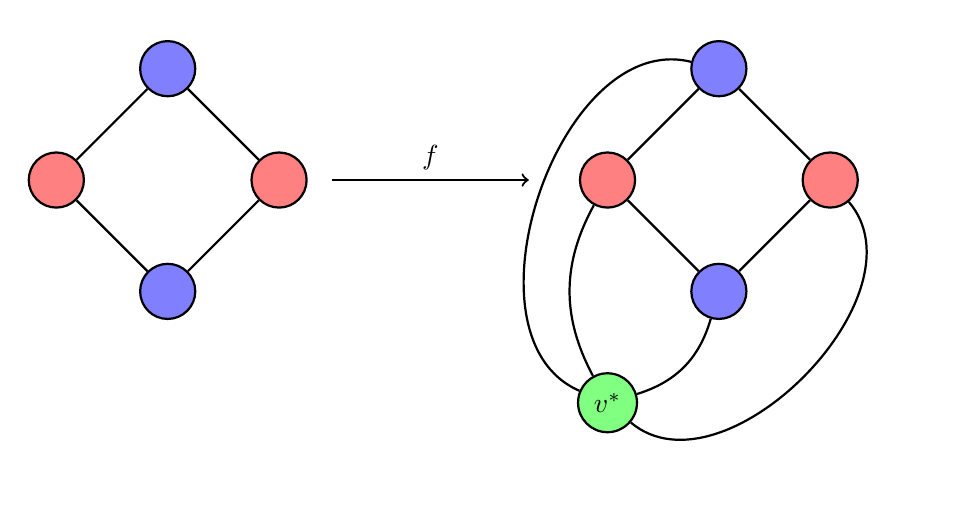
\begin{tikzpicture}[node distance={20mm}, thick,
             main/.style = {draw, circle, minimum size=0.7cm}]
            % Nodi grafo 1
            \node[main, fill = red!50] (1) {};
            \node[main, fill = blue!50] (2) [above right of=1] {};
            \node[main, fill = red!50] (3) [below right of=2] {};
            \node[main, fill = blue!50] (4) [below left of=3] {};

            \draw[<-] (6,0) -- (3.5,0) node[midway,above] {$f$};

            % Nodi grafo 2 identico a destra 
            \node[main, fill = red!50] (5) [right of=1, xshift=5cm] {};
            \node[main, fill = blue!50] (6) [above right of=5] {};
            \node[main, fill = red!50] (7) [below right of=6] {};
            \node[main, fill = blue!50] (8) [below left of=7] {};
            \node[main, fill = green!50] (9) [below left of=8] {$v^*$};

            % Archi
            \draw (1) -- (2);
            \draw (2) -- (3);
            \draw (3) -- (4);
            \draw (4) -- (1);

            \draw (5) -- (6);
            \draw (6) -- (7);
            \draw (7) -- (8);
            \draw (8) -- (5);
            \draw[bend left = 1cm] (8) to (9);
            \draw[bend left = 3cm] (7) to (9);
            \draw[bend right = 3cm] (6) to (9);
            \draw[bend right = 1cm] (5) to (9);
        \end{tikzpicture}
    \end{figure}
    L'idea è quella di aggiungere un vertice $v^*$ al grafo $\mathcal{G}$, e collegare $v^*$ a tutti i vertici
    di $\mathcal{G}$, in modo tale che $v^*$ abbia un colore diverso da tutti gli altri vertici.
    Per costruire la funzione $f$ possiamo procedere come segue:
    \begin{itemize}
        \item Dato un grafo $\mathcal{G}$, aggiungiamo un vertice $v^*$ al grafo $\mathcal{G}$.
        \item Colleghiamo $v^*$ a tutti i vertici di $\mathcal{G}$.
        \item Assegnamo a $v^*$ un colore diverso da tutti gli altri vertici, ovvero il colore $k+1$.
    \end{itemize}
    Se $\mathcal{G}$ è \texttt{k-colorabile}, allora esiste una colorazione $c$ tale che per ogni arco
    $(u,v) \in E$ si ha $c(u) \neq c(v)$. Se aggiungiamo un vertice $v^*$ al grafo $\mathcal{G}$, e lo colleghiamo
    a tutti i vertici di $\mathcal{G}$, allora $v^*$ deve avere un colore diverso da tutti gli altri vertici, ovvero
    il colore $k+1$. Quindi, se $\mathcal{G}$ è \texttt{k-colorabile}, allora $\mathcal{G'}$ è \texttt{(k+1)-colorabile}.
    
    Se $\mathcal{G}'$ è \texttt{(k+1)-colorabile} senza perdita di generalità diciamo che il colore di $v^*$ è $k+1$.
    Poiché per ogni $v$, $c(v) \neq k+1$, $c(v) \in \{1,\dots,k\}$ e quindi $c(v) \neq c(v^*)$, ovvero tutti i vertici $v$ hanno un colore diverso
    da $v^*$. Quindi, se $\mathcal{G'}$ è \texttt{(k+1)-colorabile},
    allora $\mathcal{G}$ è \texttt{k-colorabile}.
\end{proof}